\documentclass[border=10pt]{standalone}

\usepackage{tikz}
\usepackage{tikzsymbols}
\usetikzlibrary{calc,patterns,shapes.geometric}

\def\centerarc[#1](#2)(#3:#4:#5){\draw[#1] ($(#2)+({#5*cos(#3)},{#5*sin(#3)})$) arc (#3:#4:#5);}

\begin{document}
	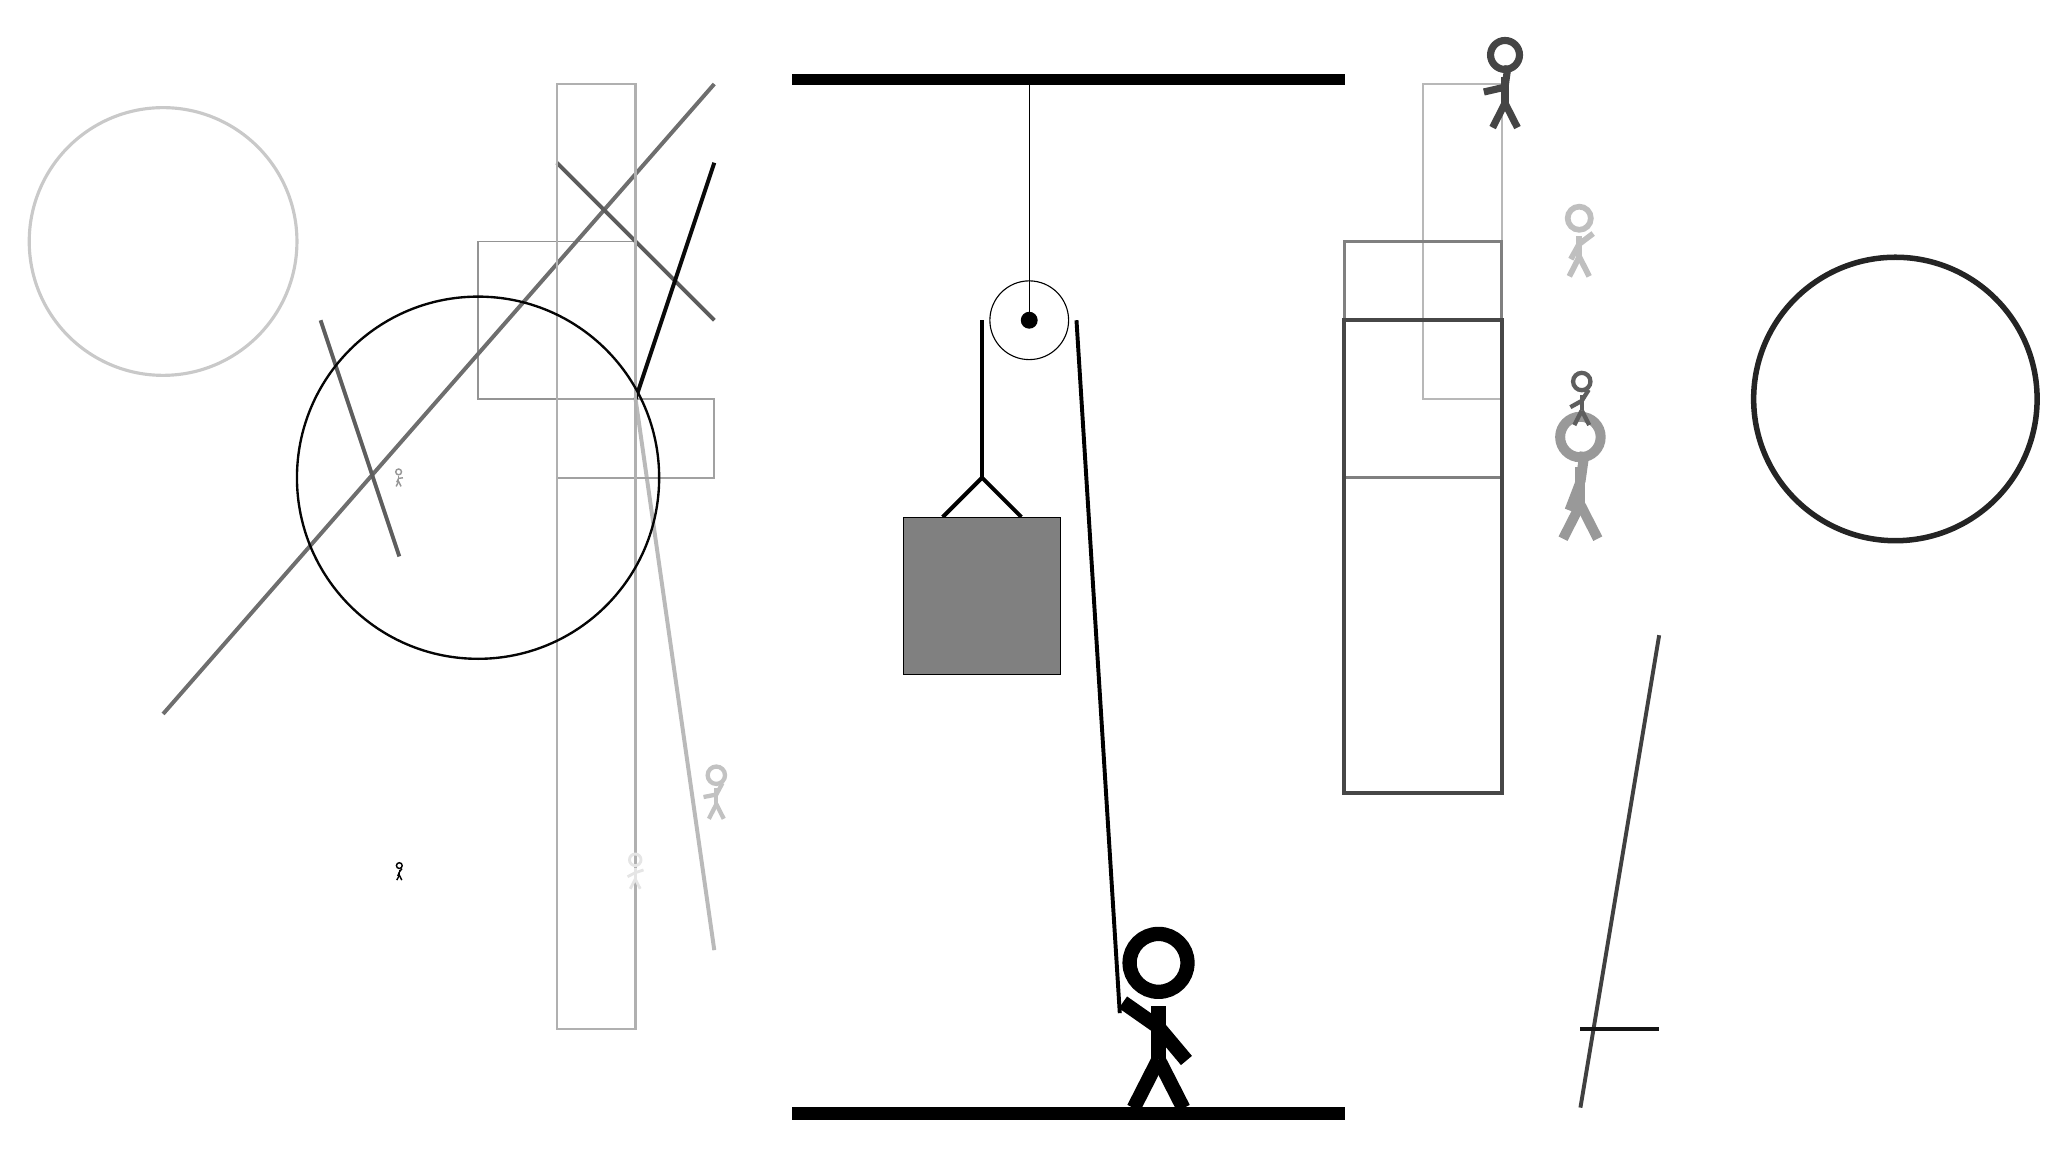
\begin{tikzpicture}
		%%%%% START %%%%%
		
		\draw[fill=black] (-2, 10) rectangle (5, 10.125);
		
		\node[line width=0.4mm, color=black!41] at (-7, 5) {\Strichmaxerl[1][64][7]};
		
		\draw[line width=0.3mm, color=black!28] (6, 6) rectangle (7, 10);
		\draw[line width=0.2mm, color=black!42] (-4, 8) rectangle (-6, 6);
		\draw[line width=0.5mm, color=black!57](-3, 10) -- (-10, 2);
		
		\node[line width=0.5mm, color=black!100] at (-7, 0) {\Strichmaxerl[1][69][52]};
		\draw [line width=0.7mm, color=black!53](10, 3) circle (0.0);
		\draw[line width=0.5mm, color=black!75](9, 3) -- (8, -3);
		
		\draw[line width=0.5mm, color=black!27](-3, -1) -- (-4, 6);
		\node[line width=0.5mm, color=black!25] at (8, 8) {\Strichmaxerl[4][61][37]};
		\draw[line width=0.2mm, color=black!37] (-3, 6) rectangle (-5, 5);
		
		\node[line width=0.6mm, color=black!24] at (-3, 1) {\Strichmaxerl[3][11][62]};
		
		\node[line width=0.4mm, color=black!40] at (8, 5) {\Strichmaxerl[7][69][82]};
		\draw[line width=0.5mm, color=black!64](-5, 9) -- (-3, 7);
		\draw[line width=0.4mm, color=black!50] (5, 8) rectangle (7, 5);
		\draw[line width=0.5mm, color=black!96](-4, 6) -- (-3, 9);
		\draw [line width=0.7mm, color=black!86](12, 6) circle (1.8);
		
		\node[line width=0.6mm, color=black!73] at (7, 10) {\Strichmaxerl[5][13][82]};
		
		\draw[line width=0.5mm, color=black!63](-7, 4) -- (-8, 7);
		\draw[line width=0.3mm, color=black!31] (-4, -2) rectangle (-5, 10);
		\draw [line width=0.4mm, color=black!21](-10, 8) circle (1.7);
		\draw[line width=0.5mm, color=black!92](8, -2) -- (9, -2);
		
		\node[line width=0.3mm, color=black!63] at (8, 6) {\Strichmaxerl[3][29][58]};
		
		\draw [line width=0.3mm, color=black!98](-6, 5) circle (2.3);
		\node[line width=0.3mm, color=black!10] at (-4, 0) {\Strichmaxerl[2][28][18]};
		\draw[line width=0.5mm, color=black!72] (5, 7) rectangle (7, 1);
		
		
		\draw (1, 7) circle (0.5);
		\draw[fill=black] (1, 7) circle (0.1);
		\draw (1, 10) -- (1, 7);
		
		\draw[line width=0.5mm] (-0.1, 4.5) -- (0.4, 5.0) -- (0.9, 4.5);
		\draw[fill=black!50] (-0.6, 4.5) rectangle (1.4, 2.5);
		
		\draw[line width=0.5mm] (0.4, 7) -- (0.4, 5.0);
		\centerarc[line width=0.5mm](1, 7)(0:180:0.6);
		\draw[line width=0.5mm](1.6, 7) -- (2.15, -1.8);
		
		\node at (2.6, -1.9) {\Strichmaxerl[10][-35][-50]};
		
		\draw[fill=black] (-2, -3) rectangle (5, -3.15);
		
		%%%%% END %%%%%
	\end{tikzpicture}
\end{document}